% Options for packages loaded elsewhere
\PassOptionsToPackage{unicode}{hyperref}
\PassOptionsToPackage{hyphens}{url}
%
\documentclass[
]{article}
\usepackage{amsmath,amssymb}
\usepackage{iftex}
\ifPDFTeX
  \usepackage[T1]{fontenc}
  \usepackage[utf8]{inputenc}
  \usepackage{textcomp} % provide euro and other symbols
\else % if luatex or xetex
  \usepackage{unicode-math} % this also loads fontspec
  \defaultfontfeatures{Scale=MatchLowercase}
  \defaultfontfeatures[\rmfamily]{Ligatures=TeX,Scale=1}
\fi
\usepackage{lmodern}
\ifPDFTeX\else
  % xetex/luatex font selection
\fi
% Use upquote if available, for straight quotes in verbatim environments
\IfFileExists{upquote.sty}{\usepackage{upquote}}{}
\IfFileExists{microtype.sty}{% use microtype if available
  \usepackage[]{microtype}
  \UseMicrotypeSet[protrusion]{basicmath} % disable protrusion for tt fonts
}{}
\makeatletter
\@ifundefined{KOMAClassName}{% if non-KOMA class
  \IfFileExists{parskip.sty}{%
    \usepackage{parskip}
  }{% else
    \setlength{\parindent}{0pt}
    \setlength{\parskip}{6pt plus 2pt minus 1pt}}
}{% if KOMA class
  \KOMAoptions{parskip=half}}
\makeatother
\usepackage{xcolor}
\usepackage[margin=1cm]{geometry}
\usepackage{color}
\usepackage{fancyvrb}
\newcommand{\VerbBar}{|}
\newcommand{\VERB}{\Verb[commandchars=\\\{\}]}
\DefineVerbatimEnvironment{Highlighting}{Verbatim}{commandchars=\\\{\}}
% Add ',fontsize=\small' for more characters per line
\usepackage{framed}
\definecolor{shadecolor}{RGB}{248,248,248}
\newenvironment{Shaded}{\begin{snugshade}}{\end{snugshade}}
\newcommand{\AlertTok}[1]{\textcolor[rgb]{0.94,0.16,0.16}{#1}}
\newcommand{\AnnotationTok}[1]{\textcolor[rgb]{0.56,0.35,0.01}{\textbf{\textit{#1}}}}
\newcommand{\AttributeTok}[1]{\textcolor[rgb]{0.13,0.29,0.53}{#1}}
\newcommand{\BaseNTok}[1]{\textcolor[rgb]{0.00,0.00,0.81}{#1}}
\newcommand{\BuiltInTok}[1]{#1}
\newcommand{\CharTok}[1]{\textcolor[rgb]{0.31,0.60,0.02}{#1}}
\newcommand{\CommentTok}[1]{\textcolor[rgb]{0.56,0.35,0.01}{\textit{#1}}}
\newcommand{\CommentVarTok}[1]{\textcolor[rgb]{0.56,0.35,0.01}{\textbf{\textit{#1}}}}
\newcommand{\ConstantTok}[1]{\textcolor[rgb]{0.56,0.35,0.01}{#1}}
\newcommand{\ControlFlowTok}[1]{\textcolor[rgb]{0.13,0.29,0.53}{\textbf{#1}}}
\newcommand{\DataTypeTok}[1]{\textcolor[rgb]{0.13,0.29,0.53}{#1}}
\newcommand{\DecValTok}[1]{\textcolor[rgb]{0.00,0.00,0.81}{#1}}
\newcommand{\DocumentationTok}[1]{\textcolor[rgb]{0.56,0.35,0.01}{\textbf{\textit{#1}}}}
\newcommand{\ErrorTok}[1]{\textcolor[rgb]{0.64,0.00,0.00}{\textbf{#1}}}
\newcommand{\ExtensionTok}[1]{#1}
\newcommand{\FloatTok}[1]{\textcolor[rgb]{0.00,0.00,0.81}{#1}}
\newcommand{\FunctionTok}[1]{\textcolor[rgb]{0.13,0.29,0.53}{\textbf{#1}}}
\newcommand{\ImportTok}[1]{#1}
\newcommand{\InformationTok}[1]{\textcolor[rgb]{0.56,0.35,0.01}{\textbf{\textit{#1}}}}
\newcommand{\KeywordTok}[1]{\textcolor[rgb]{0.13,0.29,0.53}{\textbf{#1}}}
\newcommand{\NormalTok}[1]{#1}
\newcommand{\OperatorTok}[1]{\textcolor[rgb]{0.81,0.36,0.00}{\textbf{#1}}}
\newcommand{\OtherTok}[1]{\textcolor[rgb]{0.56,0.35,0.01}{#1}}
\newcommand{\PreprocessorTok}[1]{\textcolor[rgb]{0.56,0.35,0.01}{\textit{#1}}}
\newcommand{\RegionMarkerTok}[1]{#1}
\newcommand{\SpecialCharTok}[1]{\textcolor[rgb]{0.81,0.36,0.00}{\textbf{#1}}}
\newcommand{\SpecialStringTok}[1]{\textcolor[rgb]{0.31,0.60,0.02}{#1}}
\newcommand{\StringTok}[1]{\textcolor[rgb]{0.31,0.60,0.02}{#1}}
\newcommand{\VariableTok}[1]{\textcolor[rgb]{0.00,0.00,0.00}{#1}}
\newcommand{\VerbatimStringTok}[1]{\textcolor[rgb]{0.31,0.60,0.02}{#1}}
\newcommand{\WarningTok}[1]{\textcolor[rgb]{0.56,0.35,0.01}{\textbf{\textit{#1}}}}
\usepackage{graphicx}
\makeatletter
\def\maxwidth{\ifdim\Gin@nat@width>\linewidth\linewidth\else\Gin@nat@width\fi}
\def\maxheight{\ifdim\Gin@nat@height>\textheight\textheight\else\Gin@nat@height\fi}
\makeatother
% Scale images if necessary, so that they will not overflow the page
% margins by default, and it is still possible to overwrite the defaults
% using explicit options in \includegraphics[width, height, ...]{}
\setkeys{Gin}{width=\maxwidth,height=\maxheight,keepaspectratio}
% Set default figure placement to htbp
\makeatletter
\def\fps@figure{htbp}
\makeatother
\setlength{\emergencystretch}{3em} % prevent overfull lines
\providecommand{\tightlist}{%
  \setlength{\itemsep}{0pt}\setlength{\parskip}{0pt}}
\setcounter{secnumdepth}{-\maxdimen} % remove section numbering
\usepackage{amsmath}
\usepackage{mathtools}
\usepackage{amsthm}
\usepackage{color}
\usepackage{xcolor}
\usepackage{geometry}
\usepackage{enumerate}
\ifLuaTeX
  \usepackage{selnolig}  % disable illegal ligatures
\fi
\IfFileExists{bookmark.sty}{\usepackage{bookmark}}{\usepackage{hyperref}}
\IfFileExists{xurl.sty}{\usepackage{xurl}}{} % add URL line breaks if available
\urlstyle{same}
\hypersetup{
  pdftitle={Regression Analysis - STAT 482 - Exam 1: Due December 2, 2021},
  pdfauthor={Alex Towell (atowell@siue.edu)},
  hidelinks,
  pdfcreator={LaTeX via pandoc}}

\title{Regression Analysis - STAT 482 - Exam 1: Due December 2, 2021}
\author{Alex Towell
(\href{mailto:atowell@siue.edu}{\nolinkurl{atowell@siue.edu}})}
\date{}

\begin{document}
\maketitle

\newcommand{\sos}[1]{\mathrm{SS_{#1}}}
\newcommand{\ms}[1]{\mathrm{MS_{#1}}}
\newcommand{\sd}{\operatorname{sd}}
\newcommand{\var}{\operatorname{var}}
\newcommand{\expect}{\operatorname{E}}
\newcommand{\corr}{\operatorname{cor}}
\newcommand{\cov}{\operatorname{cov}}
\newcommand{\se}{\operatorname{se}}
\newcommand{\eval}[2]{\left. #1 \right\vert_{#2}}
\newcommand{\degf}[1]{\mathrm{df_{#1}}}
\newcommand{\entropy}{\operatorname{H}}
\newcommand{\param}[1]{\textcolor{blue}{\texttt{#1}}}
\newcommand{\ci}{\operatorname{CI}}

\hypertarget{problem-1}{%
\section{Problem 1}\label{problem-1}}

\begin{quote}
Experience with a certain type of plastic indicates that a relationship
exists between the hardness (measured in Brinell units) of items molded
from the plastic (response variable \(y\) ) and the elapsed time
(measured in hours) since the termination of the molding process (input
variable \(x\)). Sixteen batches of the plastic were made, and from each
batch one test item was molded. Each test item was randomly assigned to
one of the four predetermined time levels. The data is available on
Blackboard as a csv file.
\end{quote}

\hypertarget{part-a}{%
\subsection{Part (a)}\label{part-a}}

\begin{quote}
State the simple linear regression model.
\end{quote}

\hypertarget{reproduce}{%
\subsubsection{Reproduce}\label{reproduce}}

\[
  Y_i = \beta_0 + \beta_1 x_i + \epsilon_i
\] where \begin{align*}
  \epsilon_1,\ldots,\epsilon_n &\sim \mathcal{N}(0,\sigma^2)\\
  Y_i &= \text{is the $i$-th plastic hardness response (in Brinell units)}\\
  x_i &= \text{is the $i$-th elapsed molding time}.
\end{align*}

\hypertarget{part-b}{%
\subsection{Part (b)}\label{part-b}}

\begin{quote}
Provide an interpretation for the regression parameter \(\beta_1\),
stated in the context of the problem.
\end{quote}

\hypertarget{reproduce-1}{%
\subsubsection{Reproduce}\label{reproduce-1}}

\(\beta_1\) is the difference in mean plastic hardness (in Brinell
units) from a \(1\) hour increase in elapsed molding time.

\hypertarget{part-c}{%
\subsection{Part (c)}\label{part-c}}

\begin{quote}
Compute an interval estimate for \(\beta_1\).
\end{quote}

\hypertarget{output}{%
\subsubsection{Output}\label{output}}

\begin{Shaded}
\begin{Highlighting}[]
\NormalTok{dat }\OtherTok{=} \FunctionTok{read.csv}\NormalTok{(}\StringTok{"./exam1{-}1.csv"}\NormalTok{)}
\NormalTok{dat}
\end{Highlighting}
\end{Shaded}

\begin{verbatim}
##    time hardness
## 1    16      195
## 2    16      203
## 3    16      196
## 4    16      206
## 5    24      223
## 6    24      217
## 7    24      217
## 8    24      209
## 9    32      232
## 10   32      235
## 11   32      224
## 12   32      233
## 13   40      257
## 14   40      249
## 15   40      250
## 16   40      249
\end{verbatim}

\begin{Shaded}
\begin{Highlighting}[]
\CommentTok{\#dat$time = as.double(dat$time)}
\NormalTok{reg.mod }\OtherTok{=} \FunctionTok{lm}\NormalTok{(hardness }\SpecialCharTok{\textasciitilde{}}\NormalTok{ time, }\AttributeTok{data=}\NormalTok{dat)}
\FunctionTok{confint}\NormalTok{(reg.mod)}
\end{Highlighting}
\end{Shaded}

\begin{verbatim}
##                  2.5 %     97.5 %
## (Intercept) 157.299114 174.300886
## time          1.813919   2.392331
\end{verbatim}

\hypertarget{reproduce-2}{%
\subsubsection{Reproduce}\label{reproduce-2}}

A \(95\%\) confidence interval for \(\beta_1\) is \([1.814,2.392]\).

\hypertarget{part-d}{%
\subsection{Part (d)}\label{part-d}}

\begin{quote}
Compute a confidence interval for \(\mu_h\) at \(x_h = 40\) hours.
\end{quote}

\hypertarget{output-1}{%
\subsubsection{Output}\label{output-1}}

\begin{Shaded}
\begin{Highlighting}[]
\NormalTok{x.h }\OtherTok{=} \DecValTok{40}
\FunctionTok{predict}\NormalTok{(reg.mod,}\FunctionTok{data.frame}\NormalTok{(}\AttributeTok{time=}\NormalTok{x.h),}\AttributeTok{interval=}\StringTok{"confidence"}\NormalTok{)}
\end{Highlighting}
\end{Shaded}

\begin{verbatim}
##       fit      lwr      upr
## 1 249.925 245.5966 254.2534
\end{verbatim}

\hypertarget{part-e}{%
\subsection{Part (e)}\label{part-e}}

\begin{quote}
Compute a prediction interval for \(Y_{h(\text{new})}\) at \(x_h = 40\)
hours.
\end{quote}

\hypertarget{output-2}{%
\subsubsection{Output}\label{output-2}}

\begin{Shaded}
\begin{Highlighting}[]
\FunctionTok{predict}\NormalTok{(reg.mod,}\FunctionTok{data.frame}\NormalTok{(}\AttributeTok{time=}\NormalTok{x.h),}\AttributeTok{interval=}\StringTok{"predict"}\NormalTok{)}
\end{Highlighting}
\end{Shaded}

\begin{verbatim}
##       fit      lwr      upr
## 1 249.925 238.7092 261.1408
\end{verbatim}

\hypertarget{part-f}{%
\subsection{Part (f)}\label{part-f}}

\begin{quote}
Explain the difference between a confidence interval and a prediction
interval, stated in the context of the problem.
\end{quote}

\hypertarget{reproduce-3}{%
\subsubsection{Reproduce}\label{reproduce-3}}

A confidence interval is for the mean plastic hardness (in Brinell
units) for all items molded with an elapsed time of \(40\) hours.

A prediction interval is for the mean plastic hardness (in Brinell
units) for a particular item molded with an elapsed time of \(40\)
hours.

\hypertarget{part-g}{%
\subsection{Part (g)}\label{part-g}}

\begin{quote}
State the equations for \(E(\ms{R})\) and \(\ms{E}\).
\end{quote}

\hypertarget{reproduce-4}{%
\subsubsection{Reproduce}\label{reproduce-4}}

\begin{align*}
  E(\ms{R}) &= \sigma^2 + \sos{X} \beta_1^2\\
  E(\ms{E}) &= \sigma^2.
\end{align*}

\hypertarget{part-h}{%
\subsection{Part (h)}\label{part-h}}

\begin{quote}
Use part (g) to explain a motivation behind the \(F\) test for input
effects.
\end{quote}

\hypertarget{reproduce-5}{%
\subsubsection{Reproduce}\label{reproduce-5}}

Note that \[
  F^* = \frac{\ms{R}}{\ms{E}}.
\] so if \(\beta_1 \approx 0\), then \(E(\ms{R}) = E(\ms{E})\). Small
\(F^*\) indicates data compatible with the null model. Large \(F^*\)
indicates data supporting the alternative model.

\hypertarget{part-i}{%
\subsection{Part (i)}\label{part-i}}

\begin{quote}
Compute the \(F^*\) statistic and the \(p\)-value. Provide an
interpretation of the result, stated in the context of the problem.
\end{quote}

\hypertarget{output-3}{%
\subsubsection{Output}\label{output-3}}

\begin{Shaded}
\begin{Highlighting}[]
\FunctionTok{anova}\NormalTok{(reg.mod)}
\end{Highlighting}
\end{Shaded}

\begin{verbatim}
## Analysis of Variance Table
## 
## Response: hardness
##           Df Sum Sq Mean Sq F value    Pr(>F)    
## time       1 5661.6  5661.6  243.27 3.033e-10 ***
## Residuals 14  325.8    23.3                      
## ---
## Signif. codes:  0 '***' 0.001 '**' 0.01 '*' 0.05 '.' 0.1 ' ' 1
\end{verbatim}

\hypertarget{reproduce-6}{%
\subsubsection{Reproduce}\label{reproduce-6}}

Since \(p\)-value \(= .000\), the data is not compatible with the no
effect model. We accept the model which includes elapsed molding time as
a predictor of hardness.

\hypertarget{part-j}{%
\subsection{Part (j)}\label{part-j}}

\begin{quote}
Compute the coefficient of determination \(r^2\). Provide an
interpretation of the result, stated in the context of the problem.
\end{quote}

\hypertarget{output-4}{%
\subsubsection{Output}\label{output-4}}

\begin{Shaded}
\begin{Highlighting}[]
\FunctionTok{summary}\NormalTok{(reg.mod)}\SpecialCharTok{$}\NormalTok{r.squared}
\end{Highlighting}
\end{Shaded}

\begin{verbatim}
## [1] 0.9455819
\end{verbatim}

\hypertarget{reproduce-7}{%
\subsubsection{Reproduce}\label{reproduce-7}}

We estimate that \(95\%\) of the variation in hardness is explained by
elapsed molding.

\hypertarget{part-k}{%
\subsection{Part (k)}\label{part-k}}

\begin{quote}
State the full model (saturated model) in testing for regression model
fit.
\end{quote}

\hypertarget{reproduce-8}{%
\subsubsection{Reproduce}\label{reproduce-8}}

There are \(c=4\) levels of the input (predictor) variable \(x\) (time)
where the \(i\)-th level of \(x\) has \(n_i = 4\) replications for
\(i=1,\ldots,c\).

The saturated model is given by \[
  Y_{i j} = \mu_i + \epsilon_{i j}
  \begin{cases}
    i = 1,\ldots,c\\
    j = 1,\ldots,n_i.
  \end{cases}
\] where \begin{align*}
  \epsilon_{i j} &\overset{\text{iid}}{\sim} \mathcal{N}(0,\sigma^2)\\
  \mu_i          &= \text{mean of response at the $i$-th level of $x$}\\
  Y_{i j}        &= \text{$j$-th response at the $i$-th level of $x$}.
\end{align*}

\hypertarget{part-l}{%
\subsection{Part (l)}\label{part-l}}

\begin{quote}
Compute \(\sos{PE}\) and \(\sos{LF}\) for testing the fit of the linear
regression model.
\end{quote}

\hypertarget{output-5}{%
\subsubsection{Output}\label{output-5}}

\begin{Shaded}
\begin{Highlighting}[]
\NormalTok{dat}\SpecialCharTok{$}\NormalTok{fact.time }\OtherTok{=} \FunctionTok{as.factor}\NormalTok{(dat}\SpecialCharTok{$}\NormalTok{time)}

\NormalTok{sat.mod }\OtherTok{=} \FunctionTok{lm}\NormalTok{(hardness }\SpecialCharTok{\textasciitilde{}}\NormalTok{ fact.time }\SpecialCharTok{{-}} \DecValTok{1}\NormalTok{, }\AttributeTok{data=}\NormalTok{dat)}
\FunctionTok{anova}\NormalTok{(reg.mod,sat.mod)}
\end{Highlighting}
\end{Shaded}

\begin{verbatim}
## Analysis of Variance Table
## 
## Model 1: hardness ~ time
## Model 2: hardness ~ fact.time - 1
##   Res.Df    RSS Df Sum of Sq      F Pr(>F)
## 1     14 325.82                           
## 2     12 299.75  2    26.075 0.5219 0.6062
\end{verbatim}

\hypertarget{reproduce-9}{%
\subsubsection{Reproduce}\label{reproduce-9}}

From the output, we see that \(\sos{PE} = 299.75\) and
\(\sos{LF} = 26.075\).

\hypertarget{part-m}{%
\subsection{Part (m)}\label{part-m}}

\begin{quote}
Compute the \(F_{LF}\) statistic and the \(p\)-value. Provide an
interpretation of the result, stated in the context of the problem.
\end{quote}

\hypertarget{output-6}{%
\subsubsection{Output}\label{output-6}}

See output for part (l).

\hypertarget{reproduce-10}{%
\subsubsection{Reproduce}\label{reproduce-10}}

From the output, we see that \[
  F_{LF} = \frac{\sos{LF}/(c-2)}{\sos{PE}/(n-c)} = \frac{\sos{LF}/(4-2)}{\sos{PE}/(16-4)} = \frac{26.075/2}{299.75/12} = .5219
\] which has a \(p\)-value \(= .606\).

Since the \(p\)-value is so large (small \(F_{LF}\) value), the
experiment finds that the data is compatible with the null model (linear
regression model).

\hypertarget{part-n}{%
\subsection{Part (n)}\label{part-n}}

\begin{quote}
Create a plot comparing the fitted values from the regression model with
the fitted values from the saturated model.
\end{quote}

\hypertarget{output-7}{%
\subsubsection{Output}\label{output-7}}

\begin{Shaded}
\begin{Highlighting}[]
\FunctionTok{plot}\NormalTok{(}\FunctionTok{sort}\NormalTok{(dat}\SpecialCharTok{$}\NormalTok{time),}
\NormalTok{     sat.mod}\SpecialCharTok{$}\NormalTok{fitted.values[}\FunctionTok{order}\NormalTok{(dat}\SpecialCharTok{$}\NormalTok{time)],}
     \AttributeTok{type =} \StringTok{"b"}\NormalTok{,}
     \AttributeTok{ylab =} \StringTok{"hardness"}\NormalTok{,}
     \AttributeTok{xlab =} \StringTok{"elapsed time"}\NormalTok{,}
     \AttributeTok{ylim =} \FunctionTok{c}\NormalTok{(}\FunctionTok{min}\NormalTok{(dat}\SpecialCharTok{$}\NormalTok{hardness),}\FunctionTok{max}\NormalTok{(dat}\SpecialCharTok{$}\NormalTok{hardness)))}
\FunctionTok{abline}\NormalTok{(reg.mod}\SpecialCharTok{$}\NormalTok{coefficients,}\AttributeTok{col=}\StringTok{"red"}\NormalTok{)}
\FunctionTok{points}\NormalTok{(dat}\SpecialCharTok{$}\NormalTok{time,dat}\SpecialCharTok{$}\NormalTok{hardness,}\AttributeTok{pch=}\DecValTok{16}\NormalTok{)}
\end{Highlighting}
\end{Shaded}


\includegraphics{exam1_files/figure-latex/unnamed-chunk-8-1.pdf}

\hypertarget{part-o}{%
\subsection{Part (o)}\label{part-o}}

\begin{quote}
Explain an advantage of using the regression estimate \(\hat{\mu}_{40}\)
instead of the sample mean \(\bar{y}_{40}\) and explain when this
advantage will lead to a more accurate estimator.
\end{quote}

\hypertarget{reproduce-11}{%
\subsubsection{Reproduce}\label{reproduce-11}}

Advantage of \(\hat\mu_{40}\) over \(\bar{y}_{40}\): The linear
regression estimate of a mean will have smaller variance than the
saturated model estimate. When more accurate: If the linear regression
model is appropriate, then its estimate \(\hat\mu_{40}\) will also have
a small bias.

\hypertarget{problem-2}{%
\section{Problem 2}\label{problem-2}}

\begin{quote}
Measurements were made on men involved in a physical fitness course. The
input variables under consideration are age (in years), weight (in kgs),
time to run 1.5 miles (in minutes), heart rate while resting (in bpm),
heart rate while running, and maximum heart rate. The goal is to
determine which input variables are needed to model the oxygen uptake
rate (ml/kg body weight per minute). The data is available on Blackboard
as a csv file.
\end{quote}

\hypertarget{part-a-1}{%
\subsection{Part (a)}\label{part-a-1}}

\begin{quote}
Describe the goal of the discrepancy function approach to model
selection. How is the best model defined? What are the two sources of
model error?
\end{quote}

The goal of model selection is to choose the ``best'' model from a
candidate class of models.

We consider the best model that which provides the most accurate
estimation of \(E(Y_i|x_i) = \mu_i\) at the observed input levels
\(\underbar{x}_1,\ldots,\underbar{x}_n\).

The two sources of model error are model misspecification (bias) and
parameter estimation (variance).

\hypertarget{part-b-1}{%
\subsection{Part (b)}\label{part-b-1}}

\begin{quote}
Plot the \(C_p\) statistic against the model dimension. Plot the \(C_p\)
statistic against the candidate models. Which variables are included in
the selected model?
\end{quote}

\hypertarget{output-8}{%
\subsubsection{Output}\label{output-8}}

\begin{Shaded}
\begin{Highlighting}[]
\FunctionTok{library}\NormalTok{(leaps)}
\NormalTok{dat2 }\OtherTok{=} \FunctionTok{read.csv}\NormalTok{(}\StringTok{"./exam1{-}2.csv"}\NormalTok{)}
\NormalTok{dat2}
\end{Highlighting}
\end{Shaded}

\begin{verbatim}
##    age weight runtime rstpulse runpulse maxpulse      oxy
## 1   44  89.47   11.37       62      178      182 41.05617
## 2   40  75.07   10.07       62      185      185 48.68738
## 3   44  85.84    8.65       45      156      168 57.72057
## 4   42  68.15    8.17       40      166      172 59.51438
## 5   38  89.02    9.22       55      178      180 52.34193
## 6   47  77.45   11.63       58      176      176 45.30553
## 7   40  75.98   11.95       70      176      180 44.56676
## 8   43  81.19   10.85       64      162      170 50.19773
## 9   44  81.42   13.08       63      174      176 40.44744
## 10  38  81.87    8.63       48      170      186 54.99462
## 11  44  73.03   10.13       45      168      168 49.84048
## 12  45  87.66   14.03       56      186      192 37.94971
## 13  45  66.45   11.12       51      176      176 47.01984
## 14  47  79.15   10.60       47      162      164 47.77988
## 15  54  83.12   10.33       50      166      170 46.16785
## 16  49  81.42    8.95       44      180      185 51.31369
## 17  51  69.63   10.95       57      168      172 50.17241
## 18  51  77.91   10.00       48      162      168 51.36121
## 19  48  91.63   10.25       48      162      164 50.38991
## 20  49  73.37   10.08       67      168      168 46.90032
## 21  57  73.37   12.63       58      174      176 38.82112
## 22  54  79.38   11.17       62      156      165 42.99687
## 23  52  76.32    9.63       48      164      166 45.64238
## 24  50  70.87    8.92       48      146      155 53.98943
## 25  51  67.25   11.08       48      172      172 42.68997
## 26  54  91.63   12.88       44      168      172 37.45437
## 27  51  73.71   10.47       59      186      188 44.42336
## 28  57  59.08    9.93       49      148      155 54.26127
## 29  49  76.32    9.40       56      186      188 47.82479
## 30  48  61.24   11.50       52      170      176 48.86472
## 31  52  82.78   10.50       53      170      172 39.39456
\end{verbatim}

\begin{Shaded}
\begin{Highlighting}[]
\FunctionTok{colnames}\NormalTok{(dat2) }\OtherTok{=} \FunctionTok{c}\NormalTok{(}\StringTok{"x1"}\NormalTok{,}\StringTok{"x2"}\NormalTok{,}\StringTok{"x3"}\NormalTok{,}\StringTok{"x4"}\NormalTok{,}\StringTok{"x5"}\NormalTok{,}\StringTok{"x6"}\NormalTok{,}\StringTok{"y"}\NormalTok{)}
\FunctionTok{head}\NormalTok{(dat2)}
\end{Highlighting}
\end{Shaded}

\begin{verbatim}
##   x1    x2    x3 x4  x5  x6        y
## 1 44 89.47 11.37 62 178 182 41.05617
## 2 40 75.07 10.07 62 185 185 48.68738
## 3 44 85.84  8.65 45 156 168 57.72057
## 4 42 68.15  8.17 40 166 172 59.51438
## 5 38 89.02  9.22 55 178 180 52.34193
## 6 47 77.45 11.63 58 176 176 45.30553
\end{verbatim}

\begin{Shaded}
\begin{Highlighting}[]
\NormalTok{full.mod }\OtherTok{=} \FunctionTok{regsubsets}\NormalTok{(y }\SpecialCharTok{\textasciitilde{}}\NormalTok{ ., }\AttributeTok{data=}\NormalTok{dat2)}
\NormalTok{sel }\OtherTok{=} \FunctionTok{summary}\NormalTok{(full.mod)}
\FunctionTok{plot}\NormalTok{(sel}\SpecialCharTok{$}\NormalTok{cp,}\AttributeTok{xlab=}\StringTok{"\#(variables)"}\NormalTok{,}\AttributeTok{ylab=}\StringTok{"Cp"}\NormalTok{,}\AttributeTok{type=}\StringTok{"l"}\NormalTok{,}\AttributeTok{main=} \StringTok{"Cp vs dimension"}\NormalTok{)}
\NormalTok{star }\OtherTok{=} \FunctionTok{which.min}\NormalTok{(sel}\SpecialCharTok{$}\NormalTok{cp)}
\FunctionTok{points}\NormalTok{(star,sel}\SpecialCharTok{$}\NormalTok{cp[star],}\AttributeTok{col=}\StringTok{"red"}\NormalTok{,}\AttributeTok{pch=}\DecValTok{20}\NormalTok{,}\AttributeTok{cex=}\DecValTok{2}\NormalTok{)}
\end{Highlighting}
\end{Shaded}


\includegraphics{exam1_files/figure-latex/unnamed-chunk-9-1.pdf}

\begin{Shaded}
\begin{Highlighting}[]
\FunctionTok{plot}\NormalTok{(full.mod,}\AttributeTok{scale=}\StringTok{"Cp"}\NormalTok{)}
\end{Highlighting}
\end{Shaded}

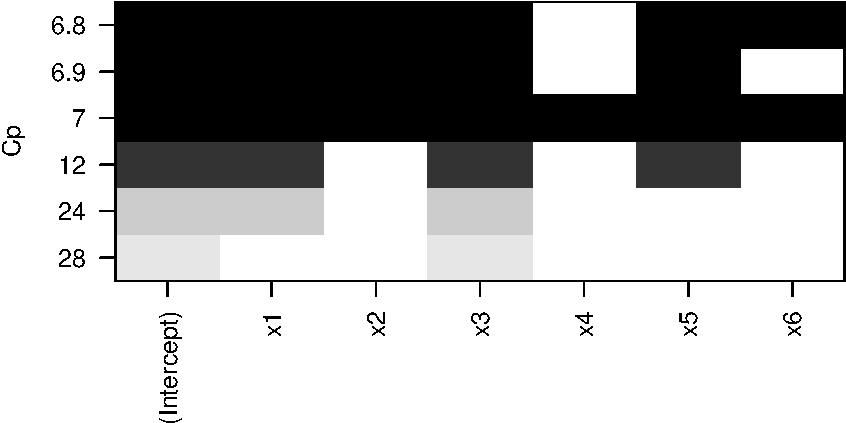
\includegraphics{exam1_files/figure-latex/unnamed-chunk-9-2.pdf}

\hypertarget{reproduce-12}{%
\subsubsection{Reproduce}\label{reproduce-12}}

We select the model which includes \(5\) input variables, \begin{align*}
  x_1 &= \text{age},\\
  x_2 &= \text{weight},\\
  x_3 &= \text{run time},\\
  x_5 &= \text{run pulse},\\
  x_6 &= \text{max pulse}.
\end{align*}

\hypertarget{part-c-1}{%
\subsection{Part (c)}\label{part-c-1}}

\begin{quote}
Test the selected model against its best competitor having fewer
parameters. (Compute the test statistic and the \(p\)-value.) How does
discrepancy based model selection compare to \(p\)-value based
selection?
\end{quote}

\hypertarget{output-9}{%
\subsubsection{Output}\label{output-9}}

\begin{Shaded}
\begin{Highlighting}[]
\NormalTok{m.R }\OtherTok{=} \FunctionTok{lm}\NormalTok{(y }\SpecialCharTok{\textasciitilde{}}\NormalTok{ x1}\SpecialCharTok{+}\NormalTok{x2}\SpecialCharTok{+}\NormalTok{x3}\SpecialCharTok{+}\NormalTok{x5, }\AttributeTok{data=}\NormalTok{dat2)}
\NormalTok{m.F }\OtherTok{=} \FunctionTok{lm}\NormalTok{(y }\SpecialCharTok{\textasciitilde{}}\NormalTok{ x1}\SpecialCharTok{+}\NormalTok{x2}\SpecialCharTok{+}\NormalTok{x3}\SpecialCharTok{+}\NormalTok{x5}\SpecialCharTok{+}\NormalTok{x6, }\AttributeTok{data=}\NormalTok{dat2)}
\FunctionTok{anova}\NormalTok{(m.R,m.F)}
\end{Highlighting}
\end{Shaded}

\begin{verbatim}
## Analysis of Variance Table
## 
## Model 1: y ~ x1 + x2 + x3 + x5
## Model 2: y ~ x1 + x2 + x3 + x5 + x6
##   Res.Df    RSS Df Sum of Sq      F Pr(>F)
## 1     26 148.08                           
## 2     25 136.50  1    11.582 2.1211 0.1577
\end{verbatim}

\hypertarget{reproduce-13}{%
\subsubsection{Reproduce}\label{reproduce-13}}

The next best reduced linear regression model discards \(x_6\) (max
pulse). So, we are testing \[
  H_0 : \beta_6 = 0
\] by comparing the model \(m_F\) that includes \(x_6\) against the
reduced model \(m_R\) that discards \(x_6\). See the ANOVA output.

We see that \(F^* = 2.121\) with a \(p\)-value \(= .158\).

We see that in the hypothesis test, we find the data to be compatible
with the reduced model, since the \(F^*\) statistic has a large
\(p\)-value. So, according to this test, we would choose \(m_R\). In the
discrepancy-based model selection, we found the best model to be
\(m_F\). Thus, the rule for adding predictors/inputs to a model is less
stringent for discrepancy based model selection than for hypothesis
testing.

\end{document}
